\section{Course Overview}

ME 571: Fluid Mechanics is a lecture based class that focuses on the analysis
and kinematics of fluids through the application of the conservation equations, dimensional
analysis, and typical flow applications. The course is computation heavy and requires
a thorough understanding of the principles at play and the mathematics associated with them.
As such, fluid mechanics provides several opportunities to show the value of programming by
allowing students to focus on the principles at play rather than the advanced mathematics.

Due to the complexity of many problems in fluid mechanics, many software packages have been
created to relieve the computational burden from engineers. A few examples include:

\begin{itemize}
    \item System of Equation Solvers
    \begin{itemize}
        \item The most common of which is Engineering Equation Solver (EES), a 
        solver that contains a multitude of built-in functions 
        and properties for thermal and fluid sciences \cite{ees}.
        \item Python and Excel also serve as capable equation solvers, though
        the experience is not nearly as tailored as EES.
    \end{itemize}
    \item Computational Fluid Dynamics (CFD)
    \begin{itemize}
        \item A CFD is a simulation program that uses numerical methods to solve fluid flow
        problems. They often output graphics, such as flow streamlines, that allow for
        a quick and easy analysis of the problem.
        \item Many popular CFD packages exist, such as ANSYS Fluent or SOLIDWORKS Flow Simulation.
    \end{itemize}
\end{itemize}

With software solutions being common in both industry and research, introducing students to
programmatic solution methods becomes even more important.

\section{New Assignment}

Currently, no assignments in ME 571: Fluid Mechanics make use of programming, but not for
the lack of options.
The study of fluid mechanics, as with many areas of engineering, requires the liberal 
application of differentials to solve problems and model systems. When given as
assignments, questions need to carefully crafted to ensure a symbolic solution can be found,
since finding a numerical solution is difficult and time-consuming. With the addition of
programming, however, finding a numerical solution becomes a trivial matter (assuming
standard numerical methods are appropriate for the problem).

Python has two libraries that excel at solving differentials, `sympy' 
\cite{Meurer_SymPy_symbolic_computing_2017} for symbolic solutions 
and `scipy' \cite{2020SciPy-NMeth} for numerical solutions. The following assignment adapted from 
\textit{Fundamentals of Fluid Mechanics, 7th Edition} \cite{fluid-mechanics}, 
Assignment \ref{fluid_assignment_1} below, shows an example of using both sympy and scipy 
to solve a question that requires both
symbolic and numerical differentials. 

\assignments{ME 571: Assignment 1}
\label{fluid_assignment_1}

\begin{tcolorbox}[breakable, enhanced jigsaw, title=ME 571: Assignment \ref{fluid_assignment_1}, 
    colframe=ksu-purple, colback=ksu-gray]

    \textbf{Problem Statement}
    \parindent15pt

    As a valve is opened, water flows through the diffuser shown in Fig. P4.31 at an increasing 
    flow rate so that the velocity along the centerline is given by 
    $ \mathbf{V} = \it{u}\mathbf{\hat{i}}  = V_0(1 - \rm{e}^{-ct})(1 - \it{x/l})\mathbf{\hat{i}} $, 
    where $\it{u}$, $ \it{c} $, and $ \it{l} $ are constants. Determine the acceleration as 
    a function of $ \it{x} $ and $ \it{t} $. If $ V_0 = 10 ft/s $ and $ \it{l} = 5 $, what value 
    of $ \it{c} $ (other than $ \it{c} = 0 $) is needed to make the acceleration 0 for any 
    $ \it{x} $ at $ \it{t} = 1s $? Explain how the acceleration can be zero if the flow rate 
    is increasing with time? Be sure to leave specify all assumptions and comment on the 
    functionality of the code.

    \begin{center}
        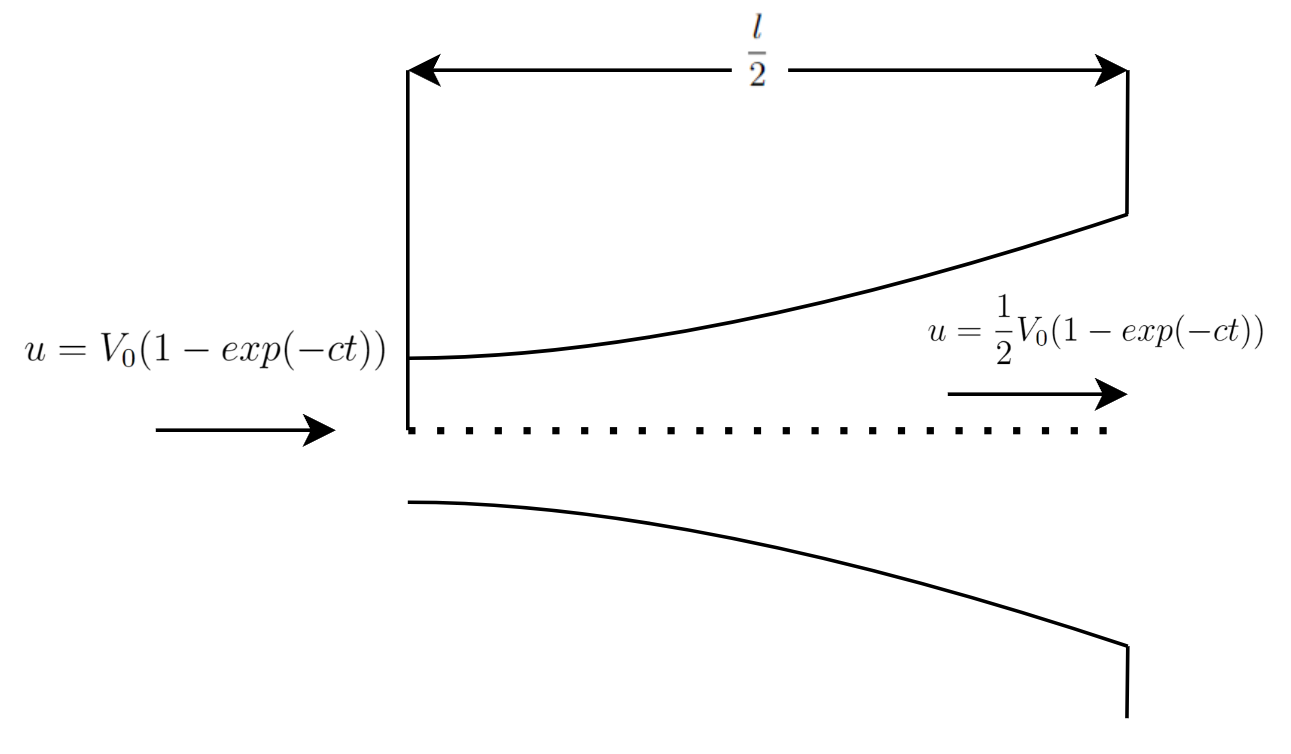
\includegraphics[width=\textwidth]{fluid-assignment1.png} 
    \end{center}

    \tcblower
    \textbf{Problem Solution}
    \parindent15pt

    For the full solution, see Appendix \ref{appendix:appendix_github}. Two solutions are 
    presented in the repository, and the entirety of solution 2 is shown below.

\begin{python}
from sympy import symbols, lambdify, diff, exp
from scipy.optimize import fsolve
from matplotlib import pyplot as plt
\end{python}

After importing the necessary libraries, we can set up the symbols that represent the 
constants and variables used in the equation. After that, create an equation for the 
velocity and use the `diff' function to get the acceleration equation.

\begin{python}
c, x, t, l, v = symbols("c x t l v")
vel = v*(1 - exp(-c * t))*(1 - x/l)
accel = diff(vel, t) + vel * diff(vel, x)
\end{python}

After getting the acceleration equation, we can substitute in the known values and then 
lambdify the equation, so we can use a numerical solver on it. Since the x-value does 
not matter for this equation, we can put in any value we want. We will opt for 1.

\begin{python}
accel = accel.subs({x: 1, t: 1, l: 5, v: 10})
acceleration = lambdify([c], accel, "scipy")
\end{python}

To use the fsolve function, you need to have an initial guess at the value. To get that
estimate, graph the acceleration function and observe where it crosses the x-axis.

\begin{python}
x = linspace(0, 1)
plt.hlines(0, 0, 1)
plt.plot(x, acceleration(x))
\end{python}

\begin{center}
    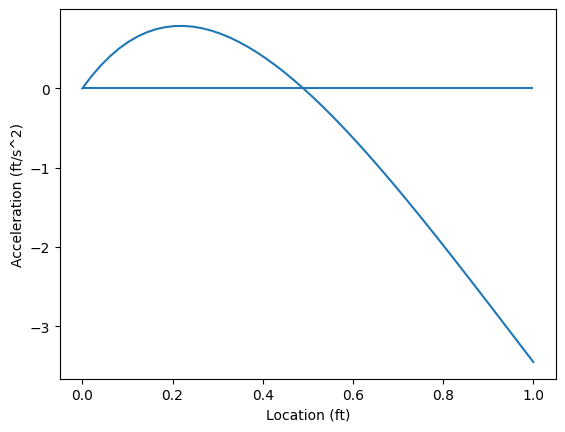
\includegraphics[scale=0.5]{fluid-plot.png}
\end{center}

Inspecting the graph shows an estimate value of 0.5. With that guess in hand, 
we can use fsolve to find the value.

\begin{python}
c = fsolve(acceleration, 0.5)
print(f"c = {c[0]:.4f} 1/s")
\end{python}

This gives an output of $ c = 0.491 \frac{1}{s} $.
\end{tcolorbox}

While the second solution is shown in Assignment \ref{fluid_assignment_1}, the first solution
assumes the student solved for the acceleration equation by hand and then used Python to
find the numerical solution.

\section{Recommendations for Course Integration}

Show in class example, provide table of everything they might need, do in class example, students now need to
understand, apply, analyze. Should assign more than once. Emphasis how common tools are used, maybe create as
a project?

\section{Project Deliverables}

In the GitHub repository associated with this paper, which can be found in 
Appendix \ref{appendix:appendix_github}, the folder titled ``7-fluid-mechanics''
contains both the problem statement and solution guide for the problem introduced in 
the previous section. The folder also contains a README that details what is in each file and 
what software is needed to complete the assignments. 

For these projects to be added to the class, the instructor would simply need to give the 
skeleton files to students as a problem statement. Given the use of specialized solving
methods used in the solution, an in-class example would be all but required.
